%TODO How to quote? Everything from github concept.md?
%TODO Part of Introduction?

\chapter{Sys-Sage}\label{chapter:sys_sage}
Sys-sage is a software library created to collect, represent and provide data on the hardware topology of HPC systems.
It is designed to extend on the existing hwloc library and provide a more versatile and dynamic use-case.

Since a lot of the hardware related data necessary for complex tasks such as thread scheduling or memory management dynamically changes during the execution of
HPC computations, the hwloc approach of providing static topology information collected on startup is often not sufficient.
Gathering the entire dataset at startup makes it difficult to incorporate user-defined data points into the topology and react to the current state of the system
such as measured bandwidth or memory usage.

Sys-sage is designed specifically to enable users to create highly customized and dynamically changeable hardware topologies and build on top of existing hwloc topologies.

\begin{figure}[ht]
    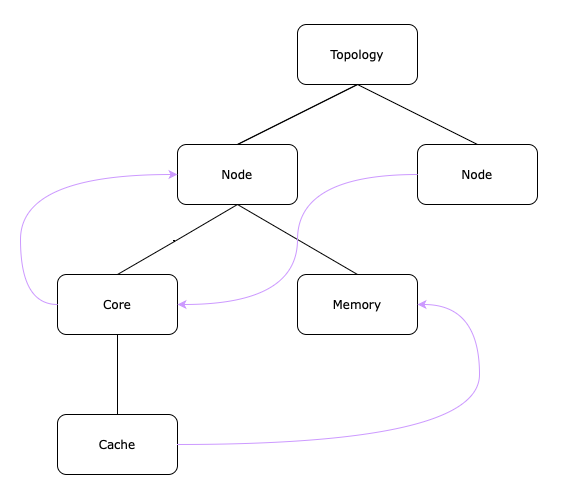
\includegraphics[scale=0.3]{images/Topology_Example.png} %TODO Improve graphic
    \centering
    \caption{Basic Component Tree with DataPaths}
    \label{figure:topology_example}
\end{figure}

The hierarchical structure of the hardware topology is represented in sys-sage as a tree of \emph{components}.
Each component corresponds to a specific part of the hardware, such as a \emph{cache, core} or \emph{node}.
Depending on the type of component, further information on the underlying hardware can be added to the component, for example the size of a cache.
Additionally, arbitrary attributes can be attached to components to provide further context or add dynamically updated values to the topology.

Beside the component tree, the \emph{DataPath} graph adds additional information to the topology.
DataPaths are connect two arbitrary components and are used to represent non-hierarchical relationships between components.
Much like components, DataPaths can have custom attributes to add additional data to component relationships.

\autoref{figure:topology_example} shows a simple example of a topology consisting of two nodes including a few components and DataPaths.